\documentclass[tikz,convert={outfile=\jobname.svg}]{standalone}
\usepackage{color}
\usepackage{tikz}

% This example lifted from
% https://dkumor.com/posts/technical/2018/08/15/causal-tikz/

% Tikz settings optimized for causal graphs.
% Just copy-paste this part
\usetikzlibrary{shapes,decorations,arrows,calc,arrows.meta,fit,positioning}
\tikzset{
    -Latex,auto,node distance =1 cm and 1 cm,semithick,
    state/.style ={ellipse, draw, minimum width = 0.7 cm},
    point/.style = {circle, draw, inner sep=0.04cm,fill,node contents={}},
    bidirected/.style={Latex-Latex,dashed},
    el/.style = {inner sep=2pt, align=left, sloped}
}
\begin{document}

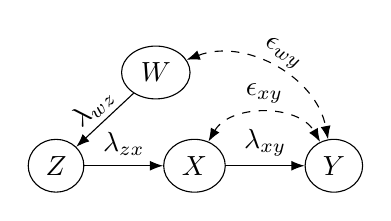
\begin{tikzpicture}
    \node[state] (1) {$Z$};
    \node[state] (2) [right =of 1] {$X$};
    \node[state] (3) [right =of 2] {$Y$};
    \node[state] (4) [above right =of 1,xshift=-0.3cm,yshift=-0.3cm] {$W$};

    \path (1) edge node[above] {$\lambda_{zx}$} (2);
    \path (2) edge node[above] {$\lambda_{xy}$} (3);
    \path[bidirected] (2) edge[bend left=60] node[above] {$\epsilon_{xy}$} (3);
    \path (4) edge node[el,above] {$\lambda_{wz}$} (1);
    \path[bidirected] (4) edge[bend left=50] node[el,above] {$\epsilon_{wy}$} (3);
\end{tikzpicture}
\end{document}
